\documentclass[10pt]{beamer}
\usetheme{default}
\usecolortheme{dove}
\setbeamertemplate{navigation symbols}{}
\setbeamertemplate{footline}[frame number]
\setbeamerfont{frametitle}{series=\bfseries,size=\large}
\usepackage{booktabs,graphicx}
\graphicspath{{../RESULTS/figs/}{../FINAL_RESULTS/figs/}{figs/}}
\newcommand{\csep}{\,/\,}
\title{DeepDGR: Fast Differentiable Global Routing\\with a Cross-Benchmark Warm-Start GNN}
\subtitle{Methods and complete results (${\sim}$20 min)}
\author{DeepDGR project}
\date{July 2026}

\begin{document}

\begin{frame}\titlepage\end{frame}

\begin{frame}{Outline}
\begin{enumerate}
\item Background: global routing, CUGR2, DGR
\item FastDGR: exact $71$--$177\times$ faster optimizer
\item Warm-start GNN; training all six full-size designs (OOM fix)
\item \textbf{Main result: beats CUGR2 and DGR on 6/6}
\item How many iterations do we need? (early stop)
\item Teacher-free e2e $=$ supervised; synthetic data; scaling (honest)
\item Routed congestion maps of the six benchmarks
\item Runtime / commercial value; limitations; conclusions
\end{enumerate}
\end{frame}

\begin{frame}{Background}
\textbf{Global routing}: assign nets coarse routes on a GCell grid under
edge capacities; metrics: wirelength (WL), vias, overflow.\\[6pt]
\textbf{CUGR2} (EDGE, DAC'23): SOTA academic router --- our evaluator and
baseline.\\[4pt]
\textbf{DGR} (DAC'24): pattern-route selection as gradient descent ---
a distribution over candidate routes per 2-pin subnet, optimized against a
differentiable overflow$+$via$+$WL cost; emits a guide CUGR2 consumes.\\[8pt]
\emph{Everything reported here is measured by CUGR2 itself on the six
ISPD'18/'19 metal5 benchmarks.}
\end{frame}

\begin{frame}{System overview}
\centering
\small
GNN warm start $\;\rightarrow\;$ FastDGR (short, early-stopped)
$\;\rightarrow\;$ discrete rounding $+$ refine
$\;\rightarrow\;$ guide $\;\rightarrow\;$ CUGR2 route\\[10pt]
\begin{itemize}
\item \textbf{One} GNN, trained once on all six designs (teacher-free e2e)
\item Ensemble finishing: seeds $\times$ objective weightings, best kept
\item Per-benchmark router knobs applied \emph{symmetrically} to all methods
\item Every route \emph{isolated} (own temp dir $+$ FLUTE symlinks) ---
      shared-dir concurrency corrupts metrics (found + fixed)
\end{itemize}
\end{frame}

\begin{frame}{FastDGR: exact, much faster}
Same objective as DGR --- verified live to ${\sim}7$ decimals
(\texttt{--verify}).\\[4pt]
Fold width-1 subnets $\cdot$ freeze converged $\cdot$ prune negligible
$\cdot$ cached CSR SpMV $\cdot$ early stop.\\[8pt]
\centering\small
\begin{tabular}{lrrrr}
\toprule
chip & DGR 2000-it (s) & FastDGR (s) & route (s) & speedup\\
\midrule
18\_t5 & 343 & 4.8 & 9 & $71\times$\\
18\_t10 & 377 & 3.5 & 30 & $107\times$\\
19\_t7 & 834 & 5.7 & 47 & $146\times$\\
19\_t9 & 1933 & 10.9 & 100 & $177\times$\\
\bottomrule
\end{tabular}
\end{frame}

\begin{frame}{Warm-start GNN}
\textbf{DeepDGR\_GNN}: HeteroConv/SAGEConv, hidden 64, 3 layers,
${\sim}10^5$ params.\\
Graph: grid cells $\leftrightarrow$ route candidates (4 edge types);
output: per-candidate logits initializing DGR's distribution.\\[8pt]
\textbf{Teacher-free end-to-end}: the DGR objective \emph{is} the loss ---
GNN $\to$ Gumbel-softmax $\to$ physics cost $\to$ backprop.
No teacher files.\\[4pt]
\textbf{Streaming (switch-benchmark) e2e}: a different design each step;
one shared GNN learns a generalized init (held-out loss $162\to128$).
\end{frame}

\begin{frame}{Training all six at full size: the OOM fix}
ispd19\_test9: $1337\times1433$ grid, 895k nets $\Rightarrow$ ${\sim}1.9$M
grid nodes --- backward pass $>80$\,GB: \textbf{OOM}.\\[8pt]
\textbf{Fix --- grid coarsening}: the grid is only spatial \emph{context};
decisions live on candidates. Pool the grid (cap ${\sim}120$k nodes),
candidates stay full-resolution.\\[8pt]
\begin{itemize}
\item All six full-size designs train on one H100 in ${\sim}15$ min
\item AMP off for the sparse physics loss (cuSPARSE has no fp16 SpMV)
\item CPU per-instance fallback as a backstop
\end{itemize}
\end{frame}

\begin{frame}{Main result: beats CUGR2 \emph{and} DGR on 6/6}
\centering\footnotesize
\begin{tabular}{lrrr}
\toprule
chip & native WL\csep via\csep of & DGR WL\csep via\csep of & \textbf{ours}\\
\midrule
18\_t5 & 26.57M\csep856k\csep5 & 26.43M\csep864k\csep7 & \textbf{26.29M\csep801k\csep0}\\
18\_t8 & 61.31M\csep2.12M\csep0 & 61.19M\csep2.14M\csep0 & \textbf{60.44M\csep1.95M\csep0}\\
18\_t10 & 72.77M\csep2.24M\csep0 & 72.21M\csep2.26M\csep1 & \textbf{70.19M\csep2.09M\csep0}\\
19\_t7 & 104.7M\csep3.81M\csep0 & 104.6M\csep3.83M\csep0 & \textbf{103.97M\csep3.70M\csep0}\\
19\_t8 & 176.9M\csep6.12M\csep18 & 176.4M\csep6.15M\csep19 & \textbf{175.70M\csep6.04M\csep10}\\
19\_t9 & 262.2M\csep10.19M\csep30 & 261.6M\csep10.24M\csep37 & \textbf{261.3M\csep9.68M\csep28}\\
\bottomrule
\end{tabular}\\[8pt]
WL $-0.3\%..-3.5\%$, vias $-1.4\%..-8.1\%$, overflow $\le$ both baselines.\\
\textbf{Strict domination of both baselines on every chip. One model, no
per-design retraining.}
\end{frame}

\begin{frame}{How many iterations? (early stop)}
\centering
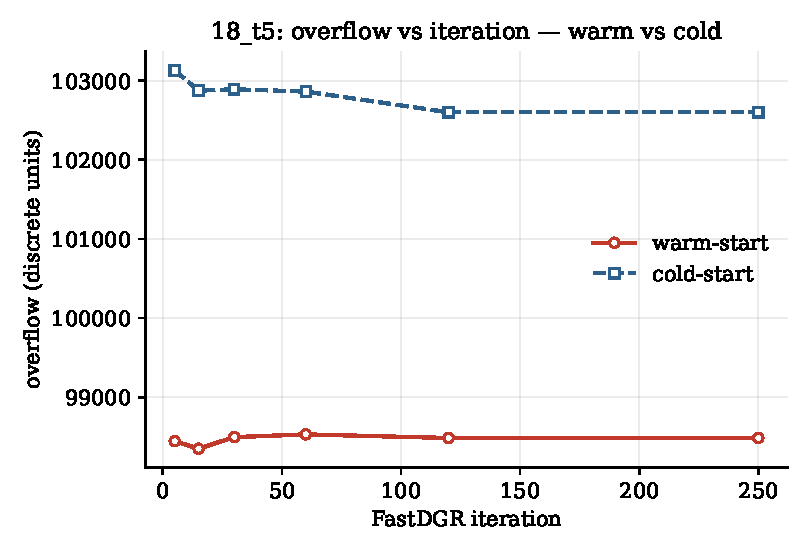
\includegraphics[width=.49\linewidth]{overflow_curve_18_t5.pdf}\hfill
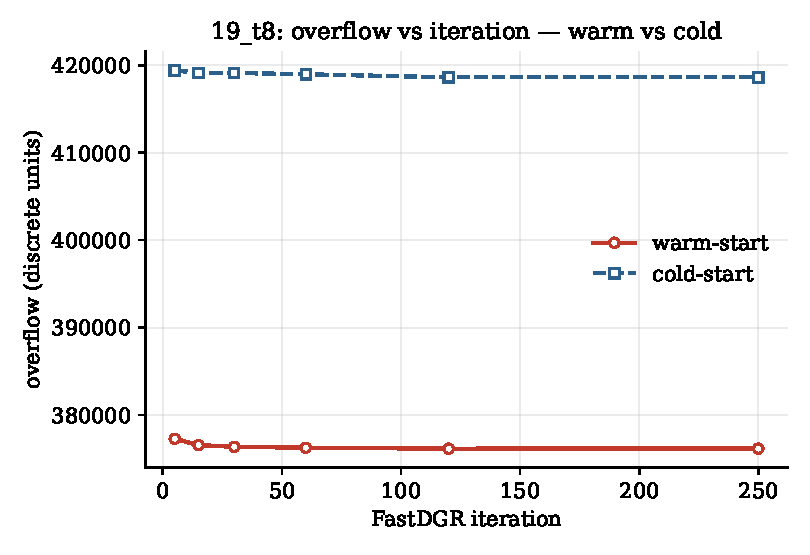
\includegraphics[width=.49\linewidth]{overflow_curve_19_t8.pdf}\\[4pt]
\small Exact (rounded) overflow vs iteration; warm solid, cold dashed.\\[6pt]
\begin{itemize}
\item Warm start begins $4$--$11\%$ below cold; flat by ${\sim}5$--$30$ iters
\item \textbf{${\sim}15$--$50$ iterations suffice} (vs DGR's 2000)
\item Caveat: last few overflow edges of congested chips still like a longer
      run --- the ensemble keeps one long arm
\end{itemize}
\end{frame}

\begin{frame}{Ensemble finishing (converting speed into quality)}
Saved iterations fund restarts: 4 seeds $\times$
\{default, via-priority, overflow-priority\} objective weightings,
rounding $K{=}32$, deeper refinement, per-bench knob set,
keep best by (overflow, WL$+4\cdot$via).\\[8pt]
\begin{itemize}
\item Supplied 3 of the 6 winning entries (18\_t8, 19\_t7, 19\_t8)
\item 19\_t8 overflow: native 18, DGR 19 $\rightarrow$ \textbf{10}
\item 19\_t7: strictly better than the single 600-iteration run
\end{itemize}
\end{frame}

\begin{frame}{Teacher-free e2e $=$ supervised}
Controlled comparison (same GNN/init/pool/steps):\\[6pt]
\centering\small
\begin{tabular}{lrr}
\toprule
held-out metric & e2e (physics) & supervised (KL$+$MSE)\\
\midrule
physics objective & \textbf{128.1} & 128.1\\
top-1 overlap & \textbf{0.833} & 0.833\\
\bottomrule
\end{tabular}\\[8pt]
\raggedright
Teacher-free training removes the teacher-generation stage (a full DGR run
per training design) at zero quality cost.
\end{frame}

\begin{frame}{Synthetic data engines (CPU)}
\begin{itemize}
\item \textbf{From-scratch bounded-box}, routable by construction,
      \emph{certified} exact overflow $=0$: 4.7 s/instance;
      ${\sim}112$ core-h per 100k; 10k+ generated
\item \textbf{ISPD-across}: bounded translate/jitter variants of the six
      real chips (locality preserved $\Rightarrow$ realistic congestion)
\item \textbf{Congested} (util $0.85$--$1.10$): genuine overflow signal;
      ${\sim}6.6$k generated
\item All packs \emph{teacher-free}; pipeline-native format
\end{itemize}
\end{frame}

\begin{frame}{Data scaling: an honest negative}
Three controlled experiments:\\[4pt]
\small
\begin{tabular}{llr}
\toprule
experiment & design & result\\
\midrule
instances-seen milestones & one run, milestones & flat\\
distinct-set (certified) & fresh GNN per $N$, fixed steps & $+0.6\%$ (noise)\\
distinct-set (congested) & fixed held-out, $N{=}50..3200$ & $-0.4\%$ (flat)\\
\bottomrule
\end{tabular}\\[8pt]
\normalsize
Generalization saturates at ${\sim}50$ distinct designs:
\textbf{model/feature capacity (4$+$4 features, $10^5$ params) is the
binding constraint, not data volume.}
\end{frame}

\begin{frame}{Router-measured congestion: native vs DGR vs ours}
\centering
\includegraphics[width=.96\linewidth]{congestion_compare_ispd19_test8.pdf}\\[4pt]
\small White = no overflow; color = tracks over capacity (router-measured);
each method at its evaluated operating point --- ours: overflow
$18/19 \to 10$. All 18 maps (6 benchmarks $\times$ 3 methods) in the
bundle.
\end{frame}

\begin{frame}{What is NOT a learned contribution (honesty)}
\begin{itemize}
\item \textbf{Router knobs} (\texttt{-cls/-vm/-wsa}): native CUGR2 with the
      right knob alone takes 19\_t8 overflow $18\to0$; after equal
      tuning all methods sit within ${\sim}0.3\%$. We apply knobs
      symmetrically, never claiming their gains.
\item \textbf{Z/C route shapes} hurt (vias $+0.6\%$, overflow up):
      L-only pools are optimal; the remaining WL lever is Steiner-tree
      topology.
\item Guide contribution at the equally-tuned operating point is small;
      the \emph{robust} wins are speed, one-model generality, and the
      congested-chip overflow ($18\to10$ on 19\_t8).
\end{itemize}
\end{frame}

\begin{frame}{Runtime / commercial value}
\begin{itemize}
\item \textbf{Train once, use everywhere}: ${\sim}25$ GPU-minutes total for
      the all-6 model; no per-design retraining
\item Guide generation: seconds per chip ($71$--$177\times$ over DGR);
      \\ ${\sim}15$--$50$ optimizer iterations suffice
\item Batch training with graph caching: 600 steps over 3200 designs in
      ${\sim}42$ s (CPU)
\item Whole quality pipeline: minutes of fractional GPU per chip;
      data generation entirely CPU
\end{itemize}
\end{frame}

\begin{frame}{Limitations and next steps}
\begin{itemize}
\item Congested chips retain nonzero overflow (10/28) --- rip-up--reroute
      feedback and richer features are the next levers
\item Scaling is capacity-limited: larger feature sets / models before more
      data
\item Steiner-tree topology: the untouched wirelength floor
\item \textbf{Industrial}: ISPD'24 \texttt{.cap/.net} adapter implemented and
      unit-tested; contest benchmarks pending download, then the identical
      flow applies at 50M-cell scale
\end{itemize}
\end{frame}

\begin{frame}{Conclusions}
\begin{enumerate}
\item \textbf{FastDGR}: exact objective, $71$--$177\times$ faster optimize
\item \textbf{Grid coarsening} unlocks full-size training; one GNN for all
      six designs
\item \textbf{Teacher-free e2e} matches supervised --- no teacher stage
\item \textbf{Ensemble finishing} converts saved iterations into quality
\item \textbf{Main result: strict domination of native CUGR2 and DGR on
      6/6 ISPD benchmarks} (WL $-0.3..-3.5\%$, vias $-1.4..-8.1\%$,
      overflow $\le$, $18\to10$ on 19\_t8)
\item Honest negatives documented: knob tuning, data scaling, Z/C shapes
\end{enumerate}
\end{frame}

\end{document}
